In this section, we analyze the factors that influence \ssmba's performance.
Due to its relatively small size (25k sentences), number of OOD domains (3), and amount of domain shift, we focus our analysis on the Baby domain within the AR-Clothing dataset.
Ablations are performed on a single domain rather than all domains, so error bars correspond to variance in models trained with different seeds and results are not comparable with those in Table \ref{tab:sent_results}.
Unless otherwise stated, we train CNN models and augment with \ssmba, corrupting 45\% of tokens, performing unrestricted sampling when reconstructing, and using self-supervised soft labelling, generating 5 synthetic examples for each training example. 

\subsection{Training Set Size}
\label{subsec:dsize_exp}
We first investigate how the size of the initial dataset affects \ssmba's effectiveness.
Since a smaller dataset covers less of the training distribution, we might expect the data generated by \ssmba\ to explore less of the data manifold and reduce its effectiveness.
We subsample 25\% of the original dataset to form a new training set, then repeat this process successively to form exponentially smaller and smaller datasets. 
The smallest dataset contains only 24 examples.
For each dataset fraction, we train 10 models and average performance,
tuning a set of \ssmba\ hyperparameters on the same ID validation data.
Figure \ref{fig:dset_exp} shows that \ssmba\ offers OOD performance gains across almost all dataset sizes, even in low resource settings with less than 100 training examples.

\begin{figure}[t]
\centering
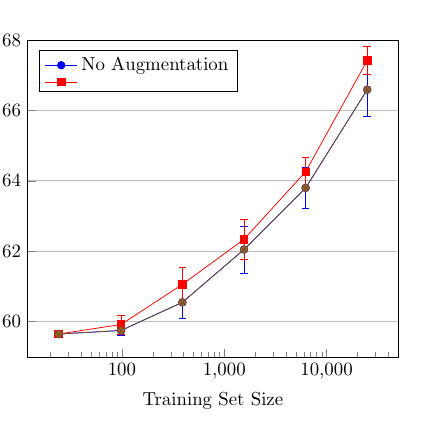
\begin{tikzpicture}[scale=0.68, trim axis left]
\begin{axis}[
    xmode=log,
    log ticks with fixed point,
    xlabel=Training Set Size,
    ylabel=OOD Accuracy (\%),
    legend pos=north west,
    xtick pos=left,
    ytick pos=left,
    ymin=59,ymax=68,
    ymajorgrids=true,
    height=7.5cm, width=8.5cm,
    % for log axes, x filter operates on LOGS.
    % and log(x * 1000) = log(x) + log(1000):
    %x filter/.code=\pgfmathparse{#1 + 6.90775527898214},
]

\addplot+[blue, mark options={blue}, error bars/.cd, y dir=both, y explicit,] table [x=x, y=y,y error=error, col sep=comma] {
    x,  y,      error
    24, 59.65, 0.02
    98,	 59.75, 0.15
    390,	60.55, 0.47
    1562,	62.05, 0.67
    6250,  63.8,       0.58
    25000, 66.59, 0.76
};
\addlegendentry{No Augmentation}

\addplot+[red, mark options={red}, error bars/.cd, y dir=both, y explicit,] table [x=x, y=y,y error=error, col sep=comma] {
    x,  y,      error
24,	59.65, 0.06
98,	 59.92, 0.27
390,	61.06, 0.47
1562,	62.34, 0.56
6250,	64.26, 0.40
25000, 67.42, 0.41
};
\addlegendentry{\ssmba}

\comment{
\addplot table {
24 59.65
98	 59.75
390	60.55
1562	62.05
6250	63.8
25000 66.59
};
}

\end{axis}
\end{tikzpicture}
\caption{OOD accuracy of models trained on successively subsampled datasets. The full training set contains 25k examples. Error bars show standard deviation in OOD accuracy across models.}
\label{fig:dset_exp}
\end{figure}



\subsection{Reconstruction Model Capacity}
\label{subsec:capacity_exp}
Since \ssmba\ relies on a reconstruction function that approximates the underlying data manifold, we might expect a larger and more expressive model to generate higher quality examples.
We investigate three models of varying size: DistilRoBERTa \citep{sanh2019distilbert} with 82M parameters, RoBERTa\textsubscript{BASE} with 125M parameters, and RoBERTa\textsubscript{LARGE} with 355M parameters. 
For each reconstruction model, we generate a set of 10 augmented datasets and train a set of 10 models on each augmented dataset. We average performance across models and datasests.
Table \ref{tab:recon_exp} shows that \ssmba\ displays robustness to the choice of reconstruction model, with all models conferring similar improvements to OOD accuracy. Using the smaller DistilRoBERTa model only degrades performance by a small margin.

\begin{table}[t]
    \small
    \centering
    \begin{tabular}{lccc}
        \toprule
        & Distil & Base & Large \\
        \midrule
        OOD Accuracy Boost (\%) & 0.73 & 0.78 & 0.78\\
        \bottomrule
    \end{tabular}
    \caption{Boost in OOD accuracy (\%) of models trained with \ssmba\ augmented data generated with different reconstruction functions.}
    \label{tab:recon_exp}
\end{table}

\comment{
\begin{table}[t]
    \small
    \centering
    \begin{tabular}{cc}
        \toprule
        & OOD Accuracy Boost (\%) \\
        \midrule
        Distil & 0.73 \\
        Base & 0.78 \\
        Large & 0.78 \\
        \bottomrule
    \end{tabular}
    \caption{Caption}
    \label{tab:my_label}
\end{table}
}

\comment{
\begin{figure}[t]
\centering
\begin{tikzpicture}[scale=0.7, trim axis left]
\begin{axis}[
    symbolic x coords={Distil, Base, Large},
    xtick=data, 
    bar width=45, 
    enlarge x limits=0.3,
    ymin=0,
    ylabel=Boost in OOD Accuracy (\%),
    xtick pos=left,
    ymajorgrids=true,
    ytick pos=left,
    height=7.5cm, width=8.5cm]
    
    \addplot[ybar,fill=blue, fill opacity=0.7,error bars/.cd, y dir=both, y explicit,] coordinates {
        (Distil, 0.73)% += (0,0.43) -= (0,0.43)
        (Base,0.78) %+= (0,0.38) -= (0,0.38)
        (Large,0.78)% += (0,0.43) -= (0,0.43)
    };
\end{axis}
\end{tikzpicture}
\caption{OOD accuracy of models trained with \ssmba\ augmented data generated with different reconstruction functions.
}
\label{fig:recon_exp}
\end{figure}
}

\begin{figure}[t]
\centering
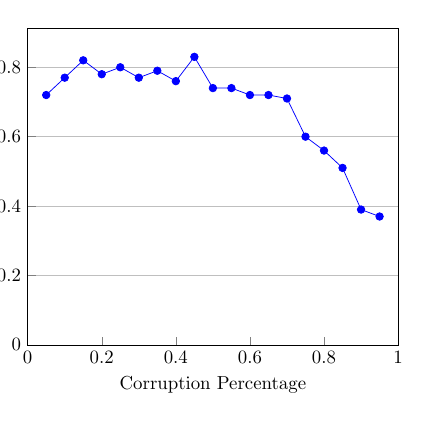
\begin{tikzpicture}[scale=0.68, trim axis left]
\begin{axis}[
    xlabel=Corruption Percentage,
    ylabel=Boost in OOD Accuracy (\%),
    xtick pos=left,
    ytick pos=left,
    ymajorgrids=true,
    xmin=0,xmax=1,
    ymin=0,
    height=7.5cm, width=8.5cm,
    % for log axes, x filter operates on LOGS.
    % and log(x * 1000) = log(x) + log(1000):
    %x filter/.code=\pgfmathparse{#1 + 6.90775527898214},
]

%\addplot[mark=none, black, dashed, ultra thick, samples=4] {66.59};
%\addlegendentry{Baseline}

\addplot+[blue, mark options={blue}] table [x=x, y=y,y error=error, col sep=comma] {
    x,  y,      error
0.05, 0.72, 0.45
0.1, 0.77, 0.39
0.15, 0.82, 0.38
0.2, 0.78, 0.44
0.25, 0.80, 0.39
0.3, 0.77, 0.37
0.35, 0.79, 0.42
0.4, 0.76, 0.37
0.45, 0.83, 0.42
0.5, 0.74, 0.39
0.55, 0.74, 0.41
0.6, 0.72, 0.41
0.65, 0.72, 0.41
0.7, 0.71, 0.42
0.75, 0.6, 0.42
0.8, 0.56, 0.42
0.85, 0.51, 0.45
0.9, 0.39, 0.47
0.95, 0.37, 0.47
};

\end{axis}
\end{tikzpicture}
\caption{Boost in OOD accuracy (\%) of models trained with \ssmba\ augmentation applied with different percentages of corrupted tokens.}
\label{fig:perturbation_exp}
\end{figure}

\subsection{Corruption Amount}
\label{subsec:noise_exp}
How sensitive is \ssmba\ to the particular amount of corruption applied?
Empirically,
tasks that were more sensitive to input noise, like sentiment analysis, required less corruption than those that were more robust, like NLI.
To analyze the effect of tuning the corruption amount, we generate 10 sets of augmented data with varying percentages of corruption, then train 10 models on each dataset, averaging performance across all 100 models.
Figure \ref{fig:perturbation_exp} shows that for corruption percentages below 50\%, our algorithm is relatively robust to the specific amount of corruption applied.
OOD performance peaks at 45\% corruption, decreasing thereafter as corruption increases.
Very large amounts of corruption tend to degrade performance, although surprisingly all augmented models still outperform unaugmented models, even when 95\% of tokens are corrupted.
In experiments on the more input sensitive NLI task, large amounts of noise degraded performance below baselines.



\subsection{Sample Generation Methods}
\label{subsec:sample_gen_exp}
Next we investigate methods for generating the reconstructed examples $\hat{x} \sim r(\hat{x}|x')$.
%Typically, the reconstruction function $r$ will generate a distribution over outputs.
%To sample $\hat{x} \sim q(\hat{x}|x')$, we investigate top-k sampling and unrestricted sampling. 
Top-k sampling draws samples from the MLM distribution on the top-k most probable tokens, leading to augmented data that explores higher probability regions of the manifold. 
We investigate top1, top5, top10, top20, and top50 sampling.
Unrestricted sampling draws samples from the full probability distribution of tokens.
This method explores a larger area of the underlying data distribution but can often lead to augmented data  in low probability regions.

For each sample generation method, we generate 5 sets of augmented data and train 10 models on each dataset.
OOD accuracy is averaged across all models for a given sampling method.
Figure \ref{fig:sample_gen_exp} shows that unrestricted sampling provides the greatest increase in OOD accuracy, with top-k sampling methods all performing similarly.
This suggests that \ssmba\ works best when it is able to explore the manifold without any restrictions.


\begin{figure}[t]
\centering
\begin{tikzpicture}[scale=0.68, trim axis left]
\begin{axis}[
    symbolic x coords={top1, top5, top10, top20, top50, unrestricted},
    xtick=data, 
    bar width=25, 
    xticklabel style={rotate=30,anchor=north east},
    %enlarge x limits=0.05,
    ylabel=Boost in OOD Accuracy (\%),
    ymin=0,
    ymajorgrids=true,
    height=7.5cm, width=8.5cm,
    xtick pos=left,
    ytick pos=left,]
    
    \addplot[ybar, fill=blue, fill opacity=0.7,error bars/.cd, y dir=both, y explicit,] coordinates {
        (top1, 0.73) +- (0, 0.4)
        (top5, 0.72) +- (0, 0.4)
        (top10,0.62) +- (0, 0.38)
        (top20,0.7) +- (0, 0.42)
        (top50,0.7) +- (0, 0.4)
        (unrestricted,0.9) +- (0, 0.41)
    };
\end{axis}
\end{tikzpicture}
\caption{Boost in OOD accuracy (\%) of models trained with \ssmba\ augmentation using different sampling methods. Error bars show standard deviation in OOD accuracy across models.}
\label{fig:sample_gen_exp}
\end{figure}

\subsection{Amount of Augmentation}
\label{subsec:aug_amount_exp}
How does OOD accuracy change as we generate more sentences and explore more of the manifold neighborhood?
To investigate we select various augmentation amounts and generate 5 datasets for each amount, training 10 models on each dataset and averaging OOD accuracy across all 50 models.
Figure \ref{fig:num_exp} shows that increasing the amount of augmentation increases the amount by which \ssmba\ improves OOD accuracy, as well as decreasing the variance in the OOD accuracy of trained models.

\begin{figure}[t]
\centering
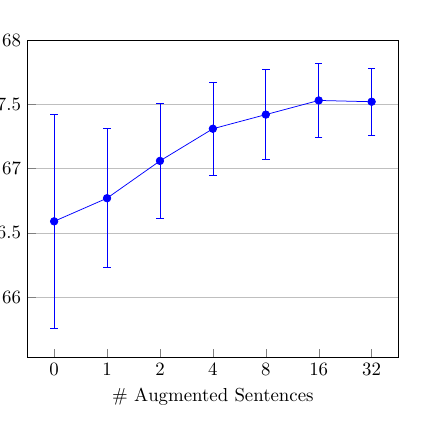
\begin{tikzpicture}[scale=0.68, trim axis left]
\begin{axis}[
    xlabel=\# Augmented Sentences,
    ylabel=OOD Accuracy (\%),
    legend pos=north east,
    xtick pos=left,
    ytick pos=left,
    xmin=-0.5, xmax=6.5,
    xticklabels={0,0,1,2,4,8,16,32},
    xtick distance=1,
    ymajorgrids=true,
    ymax=68,
    height=7.5cm, width=8.5cm,
    %ymin=66.5,ymax=67.7
    % for log axes, x filter operates on LOGS.
    % and log(x * 1000) = log(x) + log(1000):
    %x filter/.code=\pgfmathparse{#1 + 6.90775527898214},
]

\addplot[blue, mark=*, error bars/.cd, y dir=both, y explicit,] coordinates{
(0, 66.59) +- (0, 0.83)
(1, 66.77) +- (0, 0.54)
(2, 67.06) +- (0, 0.45)
(3, 67.31) +- (0, 0.36)
(4, 67.42) +- (0, 0.35)
(5, 67.53) +- (0, 0.29)
(6, 67.52) +- (0, 0.26)
};

\end{axis}
\end{tikzpicture}
\caption{OOD accuracy (\%) of models trained with different amounts of \ssmba\ augmentation. 0 augmentation corresponds to a baseline model. Error bars show standard deviation in OOD accuracy across models.}
\label{fig:num_exp}
\end{figure}



\subsection{Label Generation}
\label{subsec:label_gen_exp}
We investigate 3 methods to generate a label $\hat{y}_{ij}$ for a synthetic example $\hat{x}_{ij}$.
\textit{Label preservation} preserves the original label $y_i$.
Since the manifold neighborhood of an example may cross a decision boundary, we also investigate using a supervised model $f$ trained on the original set of unaugmented data for
\textit{hard labelling} of a one-hot class label $\hat{y}_{ij}$ and \textit{soft labelling} of a class distribution $\hat{y}_{ij}$.

We train a CNN model to varying levels of convergence and validation accuracy, then label a set of 5 augmented datasets with each labelling method.
When training with soft labels, we optimize the KL-divergence between the output distribution and soft label distribution.
For each dataset we train 10 models and average performance across all models and datasets.
Results are shown in Figure \ref{fig:label_gen_exp}.

Unsurprisingly, soft and hard labelling with a low accuracy model degrades performance.
As our supervision classifier improves, so does the performance of models trained with soft and hard labelled data.
Once we pass a certain accuracy threshold, models trained with soft labels begin outperforming all other models.
This threshold varies depending on the difficulty of the dataset and task.
In ANLI experiments, labelling augmented examples even with a poor performing model still improved downstream accuracy.

%These results suggest the heuristic of using label imputation when the initial model $f$ is poor, and using soft labelling when the initial model $f$ is strong.


\begin{figure}[t]
\centering
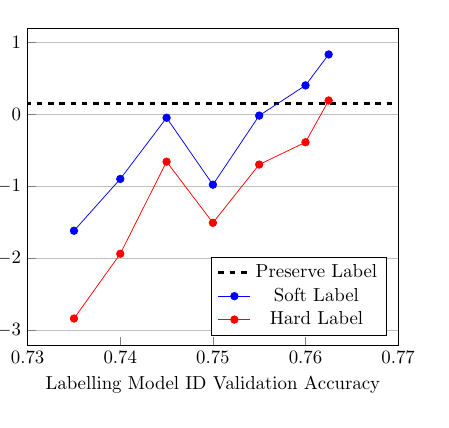
\begin{tikzpicture}[scale=0.68, trim axis left]
\begin{axis}[
    xlabel=Labelling Model ID Validation Accuracy,
    ylabel=Boost in OOD Accuracy (\%),
    legend pos=south east,
    xtick pos=left,
    ytick pos=left,
    ymajorgrids=true,
    xmin=0.73,xmax=0.77,
    height=7.5cm, width=8.5cm,
    %xmin=0,xmax=1,
    %ymin=66.5,ymax=67.7
    % for log axes, x filter operates on LOGS.
    % and log(x * 1000) = log(x) + log(1000):
    %x filter/.code=\pgfmathparse{#1 + 6.90775527898214},
]

% baseline 66.59

\addplot[mark=none, dashed, ultra thick] coordinates {(0.72,0.15) (0.78,0.15)};
\addlegendentry{Preserve Label}

\addplot [blue, mark=*] table{
0.7625 0.83
0.76 0.4
0.755 -0.02
0.75 -0.98
0.745 -0.05
0.74 -0.9
0.735 -1.62
%0.73 65.03
%0.725 64.59 
%0.715 63.6
%0.71 63.01 
%0.705 62.02
};
\addlegendentry{Soft Label}

\addplot [red, mark=*] table{
0.7625 0.19
0.76 -0.39
0.755 -0.7
0.75 -1.51
0.745 -0.66
0.74 -1.94
0.735 -2.84
%0.73 63.79
%0.725 63.55 
%0.715 62.32 
%0.71 62.04
%0.705 60.74
};
\addlegendentry{Hard Label}

\end{axis}
\end{tikzpicture}
\caption{Boost in OOD accuracy (\%) of models trained with augmented data labelled with different supervision models and label generation methods.}
\label{fig:label_gen_exp}
\end{figure}

